\documentclass{beamer}

\mode<presentation>
{
  \usetheme{default}
  \usecolortheme{default}
  \usefonttheme{default}
  \setbeamertemplate{navigation symbols}{}
  \setbeamertemplate{caption}[numbered]
  \setbeamertemplate{footline}[page number]
  \setbeamercolor{frametitle}{fg=white}
  \setbeamercolor{footline}{fg=black}
} 

\usepackage[english]{babel}
\usepackage[utf8x]{inputenc}
\usepackage{tikz}
\usepackage{listings}
\usepackage{courier}
\usepackage{array}
\usepackage{bold-extra}
\usepackage{minted}

\xdefinecolor{darkblue}{rgb}{0.1,0.1,0.7}
\xdefinecolor{darkgreen}{rgb}{0,0.5,0}
\xdefinecolor{darkgrey}{rgb}{0.35,0.35,0.35}
\xdefinecolor{darkorange}{rgb}{0.8,0.5,0}
\xdefinecolor{darkred}{rgb}{0.7,0,0}
\xdefinecolor{dianablue}{rgb}{0.18,0.24,0.31}
\definecolor{commentgreen}{rgb}{0,0.6,0}
\definecolor{stringmauve}{rgb}{0.58,0,0.82}

\lstset{ %
  backgroundcolor=\color{white},      % choose the background color
  basicstyle=\ttfamily\small,         % size of fonts used for the code
  breaklines=true,                    % automatic line breaking only at whitespace
  captionpos=b,                       % sets the caption-position to bottom
  commentstyle=\color{commentgreen},  % comment style
  escapeinside={\%*}{*)},             % if you want to add LaTeX within your code
  keywordstyle=\color{blue},          % keyword style
  stringstyle=\color{stringmauve},    % string literal style
  showstringspaces=false,
  showlines=true
}

\lstdefinelanguage{scala}{
  morekeywords={abstract,case,catch,class,def,%
    do,else,extends,false,final,finally,%
    for,if,implicit,import,match,mixin,%
    new,null,object,override,package,%
    private,protected,requires,return,sealed,%
    super,this,throw,trait,true,try,%
    type,val,var,while,with,yield},
  otherkeywords={=>,<-,<\%,<:,>:,\#,@},
  sensitive=true,
  morecomment=[l]{//},
  morecomment=[n]{/*}{*/},
  morestring=[b]",
  morestring=[b]',
  morestring=[b]"""
}

\title[2017-09-05-nanoaod-xpog]{Performance studies on NanoAOD}
\author{Jim Pivarski}
\institute{Princeton University -- DIANA}
\date{September 5, 2017}

\begin{document}

\logo{\pgfputat{\pgfxy(0.11, 8)}{\pgfbox[right,base]{\tikz{\filldraw[fill=dianablue, draw=none] (0 cm, 0 cm) rectangle (50 cm, 1 cm);}}}\pgfputat{\pgfxy(0.11, -0.6)}{\pgfbox[right,base]{\tikz{\filldraw[fill=dianablue, draw=none] (0 cm, 0 cm) rectangle (50 cm, 1 cm);}
\includegraphics[height=0.99 cm]{diana-hep-logo.png}\tikz{\filldraw[fill=dianablue, draw=none] (0 cm, 0 cm) rectangle (4.9 cm, 1 cm);}}}}

\begin{frame}
  \titlepage
\end{frame}

\logo{\pgfputat{\pgfxy(0.11, 8)}{\pgfbox[right,base]{\tikz{\filldraw[fill=dianablue, draw=none] (0 cm, 0 cm) rectangle (50 cm, 1 cm);}
\includegraphics[height=1 cm]{diana-hep-logo.png}}}}

% Uncomment these lines for an automatically generated outline.
%\begin{frame}{Outline}
%  \tableofcontents
%\end{frame}

%%%%%%%%%%%%%%%%%%%%%%%%%%%%%%%%%%%%%%%%%%%%%%%%%%%%%%%

\begin{frame}{Why I'm interested}
\vspace{0.5 cm}
NanoAOD could be the first standardized data format (across a whole experiment) that is simple enough to directly import into industry-standard tools--- Pandas, Spark, machine learning, etc.

\vspace{0.3 cm}
\begin{itemize}\setlength{\itemsep}{0.5 cm}
\item<2-> We can import complex formats (e.g.\ MiniAOD) into these frameworks by directly translating the TBranch structure to schemas, but this structure is too complicated for a data analyst to work with as-is.

\item<3-> We can also import custom formats generated by an analysis group (e.g.\ reduced TNtuples), but each of these has a limited user base.
\end{itemize}

\vspace{0.2 cm}
\uncover<4->{NanoAOD is a good candidate for a {\it centralized analysis service.}}
\end{frame}

\begin{frame}{Also, real-world test of BulkIO}
\vspace{0.5 cm}
BulkIO\footnote{See Brian Bockelman's \href{https://indico.cern.ch/event/567550/contributions/2627167/}{\textcolor{blue}{Optimizing ROOT I/O for Analysis}} at ACAT.} is a new ROOT feature (expected ROOT 6.12) that exposes purely numerical TBasket data as arrays without any copying or method calls in the loop over events.

\vspace{0.75 cm}
\uncover<2->{In the same ROOT version, I'm adding a PyROOT extension to drop the TBasket data into Numpy arrays.}

\vspace{0.25 cm}
\begin{itemize}\setlength{\itemsep}{0.5 cm}
\item<3-> streams ROOT data into Numpy-based libraries (e.g.\ Pandas, machine learning) 35$\times$ faster than current methods;
\item<4-> intended as a basis for a future query service.
\end{itemize}
\end{frame}

\begin{frame}[fragile]{First: can I read the NanoAOD?}
\vspace{0.5 cm}
Yes (as of yesterday). Interpreting underscores as structured types.

\begin{columns}
\column{1.15\linewidth}
\scriptsize
\begin{minted}{python}
List(
    MET = Record(
      phi = float32,
      pt = float32
      ),
    Muon = List(
      Record(
        charge = int32,    # electric charge
        cleanmask = uint8, # simple cleaning mask with priority to leptons
        dxy = float32,     # dxy wrt first PV, in cm
        eta = float32,
        jet = int32,       # index of the associated jet (-1 if none)
        jetPt = float32,   # pt of associated jet
        mass = float32,
        mediumId = uint8,  # POG Medium muon ID (2016 tune)
        nStations = int32, # number of matched stations with default arbitration (segment & track)
        pdgId = int32,     # PDG code assigned by the event reconstruction (not by MC truth)
        phi = float32,
        pt = float32
        )
      ),
    ...
\end{minted}
\end{columns}
\end{frame}

\begin{frame}[fragile]{Next: can I {\it use} the NanoAOD?}
Numba-compiled Python code runs on these data at MHz rates\footnote{See \href{https://arxiv.org/abs/1708.08319}{\textcolor{blue}{arXiv:1708.08319}}.}.

\begin{columns}
\column{1.1\linewidth}
\scriptsize
\begin{minted}{python}
>>> for event in events:
...     print "event", event.run, event.luminosityBlock, event.event
...     print "MET", event.MET.pt, event.MET.phi
...     for jet in event.Jet:
...         print "jet", jet.pt, jet.eta, jet.phi
...     for electron in event.Electron:
...         print "electron", electron.pt, electron.eta, electron.phi
...     print

event 1 3 1441
MET 49.6406 -2.6928
jet 46.75 1.29297 2.3437
jet 26.4375 -3.17969 0.53906
jet 25.875 -0.0688477 -0.88085
jet 21.125 3.67969 2.7812
jet 19.625 -3.33594 -1.9921
jet 17.0 -2.63281 0.99023
jet 16.6875 -3.88281 2.5390
electron 8.04297 -0.0803833 -0.85571
electron 5.53516 -0.0823364 -0.82446                                                    
\end{minted}
\end{columns}
\end{frame}

\begin{frame}{Next: what about compression?}
\vspace{0.5 cm}
Since this is an analysis-ready format, we should consider faster algorithms than LZMA.

\vspace{1 cm}
\uncover<2->{The new LZ4 algorithm trades some file size for a lot of throughput: experimental in ROOT 6.10, default in ROOT 6.12.}

\vspace{1 cm}
\uncover<3->{Will also be backported to old ROOT forks, including ROOT 5.}
\end{frame}

\begin{frame}{File size}
\begin{center}
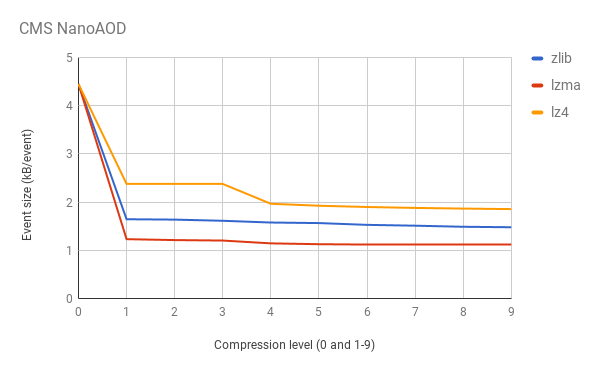
\includegraphics[width=\linewidth]{size-vs-compression.png}
\end{center}

LZMA provides the best compression; LZ4 is within a factor of 2.
\vspace{\baselineskip}
\end{frame}

\begin{frame}{Write throughput}
\begin{center}
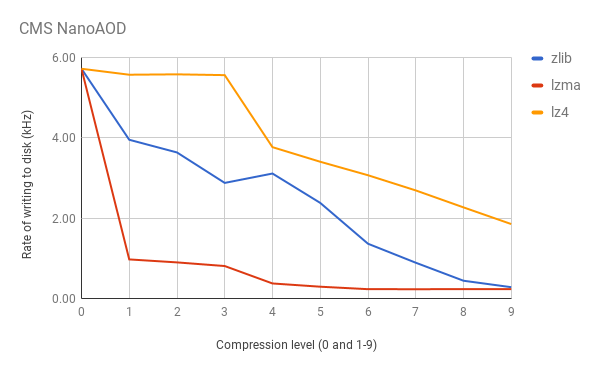
\includegraphics[width=\linewidth]{write-vs-compression.png}
\end{center}

LZ4 is fast to write: levels 1--3 have no overhead relative to {\tt TTree::CopyTree}.
\end{frame}

\begin{frame}{Read throughput (MakeClass)}
\begin{center}
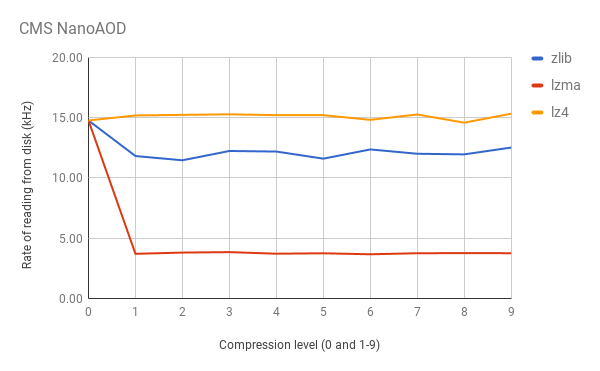
\includegraphics[width=\linewidth]{read-vs-compression.png}
\end{center}

All LZ4 levels have no overhead relative to reading data into a class generated by MakeClass. LZ4 is 4 times faster to read than LZMA.
\end{frame}

\begin{frame}{Read throughput (BulkIO: note the y-axis!)}
\begin{center}
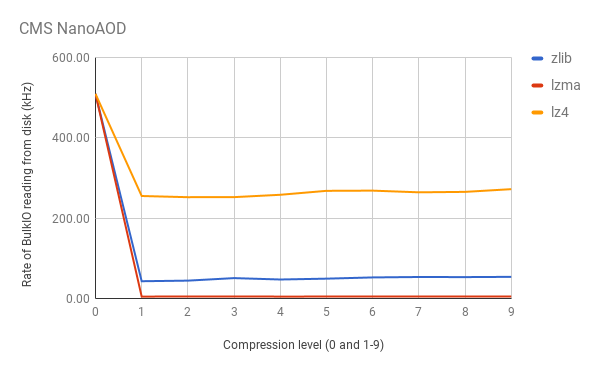
\includegraphics[width=\linewidth]{bulk-vs-compression.png}
\end{center}

BulkIO reads uncompressed data 35 times faster than filling a class; LZ4 reduces this to 17 times. LZ4 is 50 times faster than LZMA!
\end{frame}

\begin{frame}{View all as scatter plots: top-left is best}
\vspace{0.5 cm}
\begin{columns}
\column{0.38\linewidth}
\mbox{ } \hfill write vs size \hfill \mbox{ }

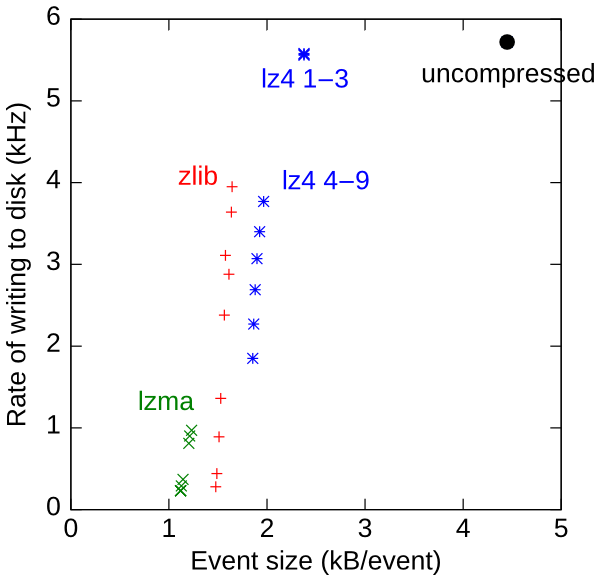
\includegraphics[width=\linewidth]{write.png}
\vspace{3 cm}
\column{0.38\linewidth}
\mbox{ } \hfill MakeClass vs size \hfill \mbox{ }

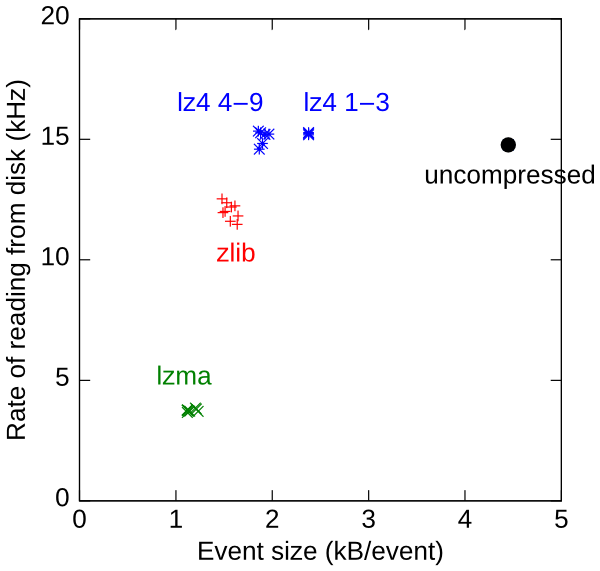
\includegraphics[width=\linewidth]{read.png}
\column{0.38\linewidth}
\vspace{3 cm}

\mbox{ } \hfill BulkIO vs size \hfill \mbox{ }

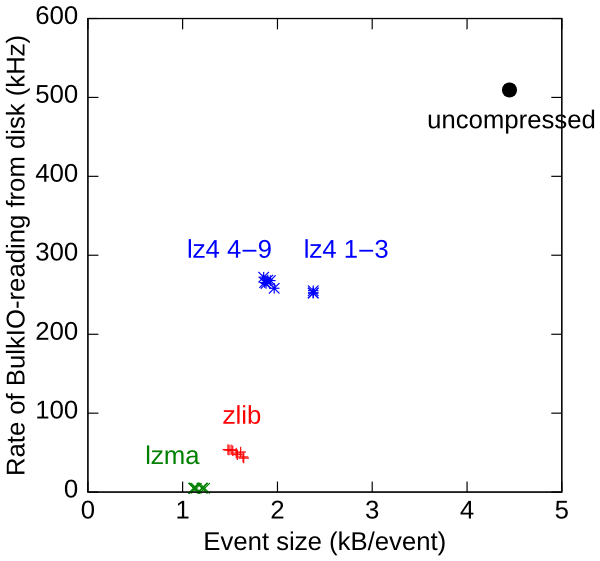
\includegraphics[width=\linewidth]{bulk.png}
\end{columns}

\vspace{-2\baselineskip}
It's about trade-offs, but the cost of \\ LZMA is very high for BulkIO!
\end{frame}

\begin{frame}{Wasted space: TBranches with counters}
\vspace{0.5 cm}
\textcolor{darkblue}{Scenario:} you want to save, e.g., arbitrarily many muons per event, so you save all the muon attributes without event boundaries and a count of the muons per event.

\vspace{0.5 cm}
\uncover<2->{ROOT does this, but it {\it also} stores indexes of the event boundaries {\it for each attribute.} This is the same data in integrated form, repeated for all attributes. Especially wasteful for rare particles with many attributes.}

\vspace{0.5 cm}
\uncover<3->{This is true for manually split objects (as in NanoAOD) and also automatically split objects (e.g.\ TClonesArray of class instances).}

\vspace{0.5 cm}
\uncover<4->{Before compression, this duplication is 10\% of NanoAOD. Can only avoid it by putting each particle type in a different TTree. Roughly corresponds to ``normal form'' in SQL.}
\end{frame}

\begin{frame}[fragile]{Working with particles in normal form}
\vspace{0.5 cm}
It's a little awkward to work with data this way in ROOT:

\vspace{0.25 cm}
\scriptsize
\begin{minted}{c++}
muoni = 0;
for (i = 0;  i < eventTree->GetEntries();  i++) {
    eventTree->GetEntry(i);      // loads nMuon

    for (j = muoni;  j < muoni + nMuon;  j++) {
        muonTree->GetEntry(j);  // loads data for one muon
        // do something with this muon
        ...

    }
    muoni += nMuon;

    // similarly for other particles...
}
\end{minted}

\vspace{0.25 cm}
\normalsize
Would we want to provide a library to facilitate this? Would that undermine the ``bare ROOT'' NanoAOD goal?

\vspace{0.25 cm}
\textcolor{gray}{(This format is no problem for Python, Spark, etc.)}
\end{frame}

\begin{frame}{File size savings of normal form: 8--18\%}
\begin{center}
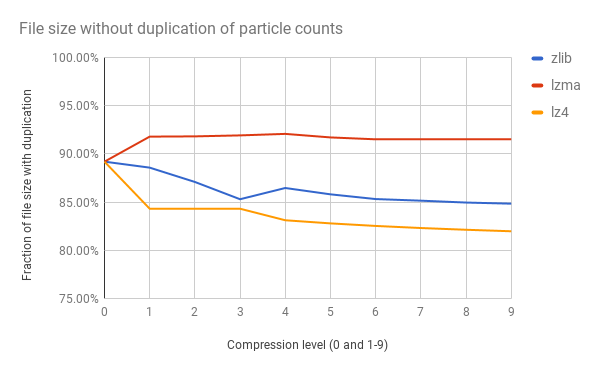
\includegraphics[width=\linewidth]{avoiding-duplication.png}
\end{center}

Because LZ4 is the worst compression algorithm for file size, it has the most to gain by not duplicating the particle count data.
\end{frame}

\begin{frame}{Total file size, now in normal form}
\begin{center}
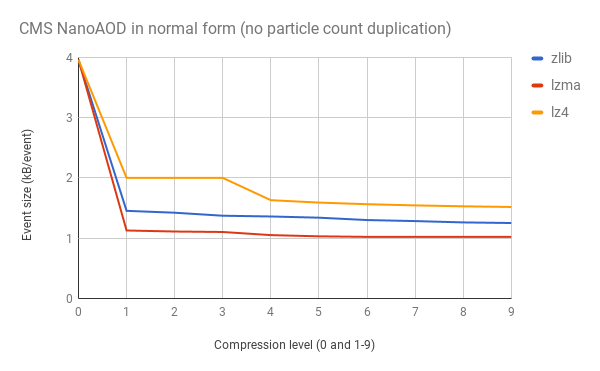
\includegraphics[width=\linewidth]{final-size.png}
\end{center}

Final ratio: LZ4 level 4 is only 1.5$\times$ bigger than LZMA level 4. \\
Much of the gap between LZ4 and LZMA was this wasted space\ldots
\end{frame}

\begin{frame}{Conclusions}
\vspace{0.5 cm}

\textcolor{darkblue}{Several technologies converging:}
\begin{itemize}\setlength{\itemsep}{0.25 cm}
\item LZ4 compression algorithm is about 50$\times$ faster than LZMA;
\item BulkIO is 35$\times$ faster than filling class objects;
\item Numpy is a good format for exposing BulkIO to Python;
\item Numba compiles Python code to restructure the data for other libraries (Pandas, PySpark, machine learning\ldots) at a rate of tens of MHz\footnote{Not shown here. See the arXiv paper.};
\end{itemize}

\vspace{0.25 cm}
\begin{itemize}
\item<2-> \ldots and NanoAOD can be the first data format published centrally by an experiment that is directly usable in these analysis tools, without intermediaries.
\end{itemize}
\end{frame}

\end{document}
